% Compile: latexmk (see README.md for PDF and print modes)
% Fonts (bundled in fonts/): Noto Sans Telugu body, Anek Telugu plain headings,
% Baloo Tammudu 2 section banners, Suravaram cover title, Ramabhadra border.
\documentclass[12pt,a4paper]{article}
\usepackage[a4paper,margin=2.2cm,top=2.8cm,bottom=2.6cm]{geometry}
\usepackage{fontspec}
\usepackage{xcolor}
\usepackage{tikz}
\newlength\covw
\newlength\covacc
\newcommand{\covfont}{\suravaram\fontsize{60}{64}\selectfont}
\usepackage{eso-pic}
\usepackage[most]{tcolorbox}
\usepackage{graphicx}
\usepackage{multicol}
\usepackage[hidelinks]{hyperref}

\defaultfontfeatures{Script=Telugu, Extension=.ttf}
\setmainfont{NotoSansTelugu}[Path=fonts/noto-sans-telugu/,
  UprightFont=*-Regular, BoldFont=*-Bold]
\newfontfamily\anek{AnekTelugu-Bold}[Path=fonts/anek-telugu/]
\newfontfamily\baloo{BalooTammudu2-Bold}[Path=fonts/baloo-tammudu-2/]
\newfontfamily\suravaram{Suravaram-Regular}[Path=fonts/suravaram/]
\newfontfamily\ramabhadra{Ramabhadra-Regular}[Path=fonts/ramabhadra/]
\linespread{1.35}
\setlength{\parindent}{0pt}
\setlength{\parskip}{0.6em}
\setlength{\emergencystretch}{3em}
\sloppy

\definecolor{saffron}{HTML}{F57C00}
\definecolor{maroon}{HTML}{8B1A1A}
\definecolor{gold}{HTML}{D4A017}
\definecolor{cream}{HTML}{FFF8E7}
\definecolor{leaf}{HTML}{2E7D32}
\definecolor{ink}{HTML}{3E2723}

\pagecolor{cream}
\color{ink}

% Corner ornaments, centred on a border corner; #2 = angle pointing into the page.
% Flower: two petal layers + leaves running along both border edges.
\newcommand{\cornerflower}[2]{%
  \begin{scope}[shift={(#1)}]
    \foreach \s in {-45,45}
      \fill[leaf,rotate=#2+\s] (0.5,0) .. controls (0.9,0.22) and (1.3,0.12) .. (1.55,0)
        .. controls (1.3,-0.12) and (0.9,-0.22) .. (0.5,0);
    \foreach \a in {0,45,...,315}
      \filldraw[fill=saffron,draw=maroon,line width=0.4pt,rotate=\a]
        (0.38,0) ellipse (0.36 and 0.16);
    \foreach \a in {22.5,67.5,...,337.5}
      \filldraw[fill=gold,draw=maroon!70,line width=0.3pt,rotate=\a]
        (0.24,0) ellipse (0.22 and 0.1);
    \filldraw[fill=maroon,draw=gold,line width=0.6pt] (0,0) circle (0.12);
  \end{scope}}
% Rangoli mandala with dotted trails along both border edges.
\newcommand{\cornermandala}[2]{%
  \begin{scope}[shift={(#1)}]
    \foreach \s in {-45,45}
      \foreach \d/\r in {0.95/0.07,1.2/0.055,1.42/0.04}
        \fill[maroon,rotate=#2+\s] (\d,0) circle (\r);
    \filldraw[fill=cream,draw=saffron,line width=1pt] (0,0) circle (0.72);
    \foreach \a in {0,30,...,330}
      \fill[gold,rotate=\a] (0.62,0) circle (0.045);
    \foreach \a in {0,45,...,315}
      \filldraw[fill=saffron!85,draw=maroon,line width=0.4pt,rotate=\a]
        (0.08,0) .. controls (0.25,0.17) and (0.45,0.1) .. (0.52,0)
        .. controls (0.45,-0.1) and (0.25,-0.17) .. (0.08,0);
    \filldraw[fill=maroon,draw=gold,line width=0.6pt] (0,0) circle (0.14);
    \fill[gold] (0,0) circle (0.05);
  \end{scope}}

% Decorative border on every page except the cover, with the title badge
% on the top edge, page number on the bottom edge and corner ornaments
% Print mode (vinayaka-vratha-kalpam-print.tex) adds a blank page after the cover
\ifdefined\printmode\def\frontpages{2}\else\def\frontpages{1}\fi
\AddToShipoutPictureBG{%
  \ifnum\value{page}>\frontpages\relax
  \begin{tikzpicture}[remember picture,overlay]
    \coordinate (NE) at ([shift={(-1.1cm,-1.1cm)}]current page.north east);
    \coordinate (SW) at ([shift={(1.1cm,1.1cm)}]current page.south west);
    \coordinate (NW) at ([shift={(1.1cm,-1.1cm)}]current page.north west);
    \coordinate (SE) at ([shift={(-1.1cm,1.1cm)}]current page.south east);
    \draw[saffron,line width=3pt,rounded corners=12pt] (SW) rectangle (NE);
    \ifodd\value{page}
      \cornerflower{NE}{225}\cornerflower{SW}{45}%
    \else
      \cornermandala{NW}{315}\cornermandala{SE}{135}%
    \fi
    \node[fill=cream,draw=saffron,line width=1.5pt,rounded corners=8pt,
      text=maroon,font=\ramabhadra,inner xsep=12pt,inner ysep=4pt]
      at ([yshift=-1.1cm]current page.north) {శ్రీ వినాయక వ్రతకల్పము};
    \node[circle,fill=saffron,text=white,inner sep=3pt,font=\small\ramabhadra]
      at ([yshift=1.1cm]current page.south) {\thepage};
  \end{tikzpicture}%
  \fi}

\pagestyle{empty}

% Telugu numerals for page numbers (expandable, so the contents page gets them too)
\newcommand\teludigit[1]{\ifcase#1 ౦\or ౧\or ౨\or ౩\or ౪\or ౫\or ౬\or ౭\or ౮\or ౯\fi}
\makeatletter
\def\telu@num#1{\ifx\relax#1\else\teludigit{#1}\expandafter\telu@num\fi}
\renewcommand\thepage{\expandafter\telu@num\number\c@page\relax}
\makeatother
% Section banner (also added to contents + PDF bookmarks)
\newcommand{\vsec}[1]{%
  \par\addvspace{0.8em}\phantomsection\addcontentsline{toc}{section}{#1}%
  \begin{tcolorbox}[enhanced,colback=saffron,colframe=maroon,boxrule=1.2pt,
    arc=6pt,halign=center,fontupper=\large\baloo\color{white},
    left=4pt,right=4pt,top=2pt,bottom=2pt,
    borderline={0.6pt}{2pt}{gold}]
    #1
  \end{tcolorbox}\nopagebreak}
% Instructions to the devotee (parenthesised notes in the original)
\newcommand{\inst}[1]{{\color{leaf}(#1)}}
% Shloka marker
\newcommand{\shl}{{\color{maroon}\bfseries శ్లో॥}}
% Count marker in the 108 names
\newcommand{\nm}[1]{\hfill{\color{saffron}\bfseries\footnotesize #1}}
% Two-panel illustration: \illus{left image}{right image}{left caption}{right caption}
\newcommand{\illus}[4]{%
  \begin{tcolorbox}[enhanced,width=0.95\textwidth,colback=white,colframe=saffron,
    boxrule=1.5pt,arc=6pt,left=3pt,right=3pt,top=3pt,bottom=3pt]
  \illuspanel{#1}{#3}\hfill\illuspanel{#2}{#4}%
  \end{tcolorbox}}
\newcommand{\illuspanel}[2]{%
  \begin{minipage}[t]{0.49\linewidth}\centering
  \includegraphics[width=\linewidth]{#1}\\[2pt]
  {\small\color{maroon}\anek #2}
  \end{minipage}}
% Telugu poem with metre label: \padya{ఉ.}{line\\line}
\newcommand{\padya}[2]{\par\noindent\makebox[2.2em][l]{\color{saffron}\bfseries #1}%
  \parbox[t]{\dimexpr\linewidth-2.2em}{#2}\par\medskip}
\newcommand{\jaya}{\hfill{\color{maroon}\bfseries ॥జ॥}}
% Highlight a verse/mantra in a soft golden box
\newtcolorbox{mantra}{enhanced,colback=gold!12,colframe=gold!80!black,
  boxrule=0.6pt,arc=4pt,left=8pt,right=8pt}

\begin{document}

% ---------------- Cover ----------------
\thispagestyle{empty}
% Syllable widths measured here: inside tikzpicture the font is nullfont
\def\covsyl{వి,నా,య,క,{\enspace},వ్ర,త,క,ల్ప,ము}
\global\covacc=0pt
\foreach \s [count=\k] in \covsyl {\settowidth\covw{\covfont\s}%
  \expandafter\xdef\csname covw\k\endcsname{\the\covw}%
  \global\advance\covacc\covw}%
\begin{tikzpicture}[remember picture,overlay]
  % Image is wider than A4: fit to page height, clip the sides
  \clip (current page.south west) rectangle (current page.north east);
  \node at (current page.center)
    {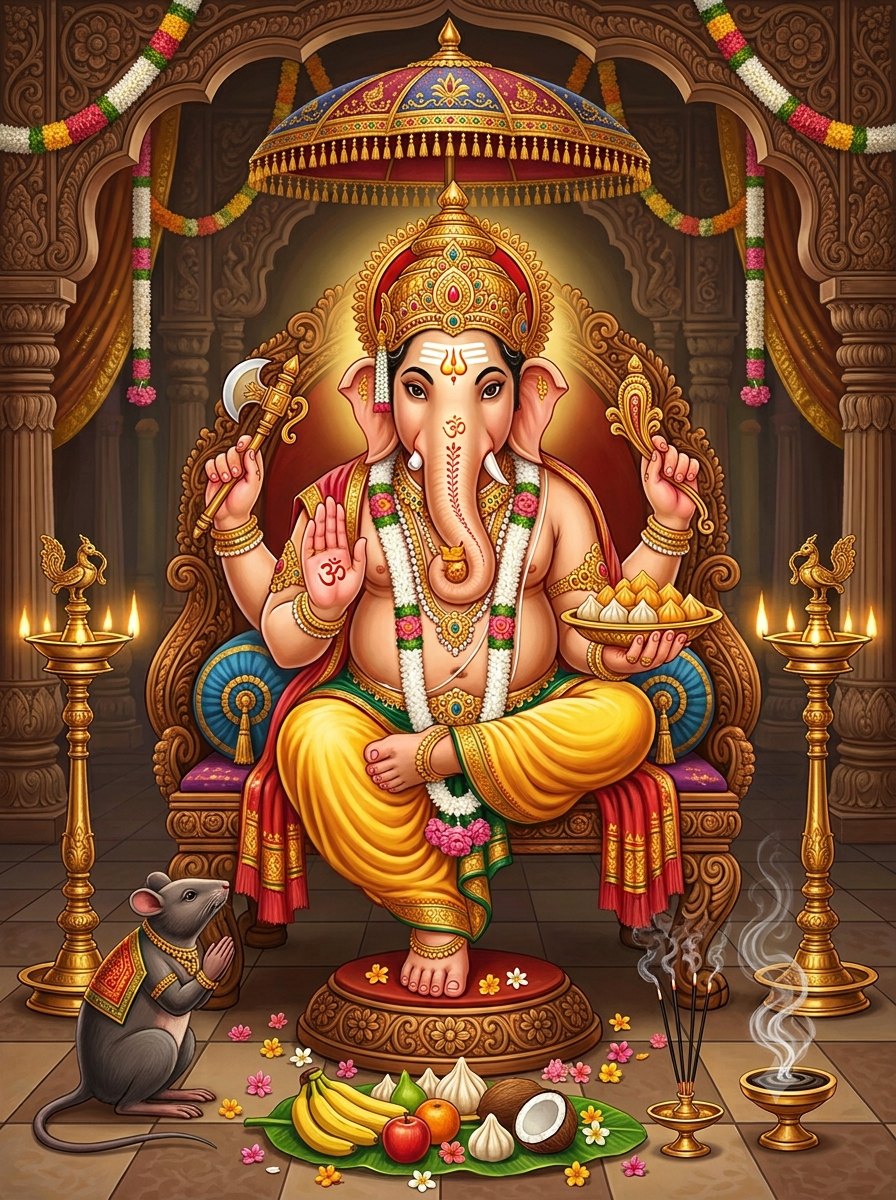
\includegraphics[height=\paperheight]{images/lord-ganesha.png}};
  % Title curved along the top of a circle. decorations.text breaks Telugu
  % conjuncts, so each syllable is its own node: widths are measured, turned
  % into angles on the arc, and the node rotated to the tangent. The maroon
  % outline is the same syllable drawn in a ring of small offsets.
  \coordinate (arcC) at ([yshift=-15.5cm]current page.north);
  \def\covR{12.8cm}
  \pgfmathsetmacro\covstart{90+deg(\covacc/(2*\covR))}
  \global\covacc=0pt
  \foreach \s [count=\k] in \covsyl {
    \covw=\csname covw\k\endcsname\relax
    \pgfmathsetmacro\ang{\covstart-deg((\covacc+0.5*\covw)/\covR)}
    \foreach \o in {0,20,...,340}
      \path (arcC) ++(\ang:\covR) ++(\o:2.6pt)
        node[anchor=base,inner sep=0,rotate=\ang-90,font=\covfont,text=maroon] {\s};
    \path (arcC) ++(\ang:\covR)
      node[anchor=base,inner sep=0,rotate=\ang-90,font=\covfont,text=yellow!85!gold] {\s};
    \global\advance\covacc\covw
  }
\end{tikzpicture}
\newpage
\ifdefined\printmode\null\newpage\fi
% ---------------- Contents ----------------
\begin{tcolorbox}[enhanced,colback=maroon,colframe=gold,boxrule=1.5pt,arc=6pt,
  halign=center,fontupper=\Large\anek\color{white}]
  విషయసూచిక
\end{tcolorbox}
{\renewcommand{\contentsname}{}\vspace{-3em}\color{maroon}\tableofcontents}
\newpage

% ---------------- Text ----------------
\begin{center}
  {\color{maroon}\anek శ్రీరస్తు}\\
  {\color{maroon}\anek శ్రీ విఘ్నేశ్వరాయ నమః}
\end{center}
\begin{tcolorbox}[enhanced,colback=maroon,colframe=gold,boxrule=2pt,arc=8pt,
  halign=center,fontupper=\LARGE\anek\color{gold!30}]
  శ్రీ సిద్ధి వినాయక వ్రతకల్పము
\end{tcolorbox}

శ్రీ-ముందుగా బొట్టు పెట్టుకుని, దీపారాధన చేసి, నమస్కరించుకుని, దిగువ విధంగా ప్రార్థించుకోవాలి.

\vsec{ప్రార్థన}
\begin{mantra}
\shl{} శుక్లాంబరధరం విష్ణుం శశివర్ణం చతుర్భుజం । ప్రసన్నవదనం ధ్యాయేత్సర్వ విఘ్నోపశాంతయే ॥
అయం ముహూర్తస్సుముహూర్తోస్తు ॥
\end{mantra}
\shl{} తదేవ లగ్నం, సుదినం తదేవ, తారాబలం చంద్రబలం తదేవ । విద్యాబలం దైవబలం తదేవ, లక్ష్మీపతే తేంఘ్రి యుగం స్మరామి ॥ సుముహూర్తోస్తు ॥
\shl{} లాభస్తేషాం జయస్తేషాం, కుతస్తేషాం పరాభవః । యేషామిందీవర శ్యామో హృదయస్థో జనార్దనః ॥
ఆపదా మపహర్తారం దాతారం సర్వ సంపదాం లోకాభిరామం శ్రీరామం భూయో భూయో నమామ్యహం ॥
సుముఖశ్చైకదంతశ్చ కపిలో గజకర్ణికః, లంబోదరశ్చ వికటో విఘ్నరాజో గణాధిపః । ధూమకేతుర్గణాధ్యక్షః ఫాలచంద్రో గజాననః వక్రతుండ శ్శూర్పకర్ణో, హేరంబః స్కంద పూర్వజః । అష్టావష్టౌ చ నామాని యః పఠేచ్ఛృణు యాదపి । విద్యారంభే వివాహేచ ప్రవేశే నిర్గమేతథా సంగ్రామే సర్వకార్యేషు విఘ్నస్తస్య నజాయతే । అభీప్సితార్థ సిద్ధ్యర్థం, పూజితోయస్సురైరపి, సర్వవిఘ్నచ్ఛిదే తస్మై గణాధిపతయే నమః ॥
\inst{నమస్కరించుకుని, ఆచమనమూ-ప్రాణాయామమూ చేసి సంకల్పము చెప్పుకొనవలెను}

\vsec{సంకల్పం}
ఓం మమోపాత్త దురితక్షయద్వారా శ్రీ పరమేశ్వర ప్రీత్యర్థం, శుభేశోభనే ముహూర్తే అద్యబ్రహ్మణః ద్వితీయపరార్థే శ్వేతవరాహకల్పే వైవస్వత మన్వంతరే కలియుగే ప్రథమపాదే, జంబూ ద్వీపే, భరతవర్షే, భరతఖండే, మేరోర్దక్షిణ దిగ్భాగే, శ్రీశైలస్య ఈశాన్యప్రదేశే, అస్మిన్ వర్తమాన వ్యావహారిక చాంద్రమానేన ప్రభవాది షష్టి సంవత్సరాణాం మధ్యే శ్రీ\ldots\ldots నామసంవత్సరే, దక్షిణాయనే, వర్షర్తౌ, భాద్రపద మాసే శుక్లపక్షే చతుర్థ్యాం తిథౌ \ldots\ldots{} వాసరయుక్తాయాం, శుభనక్షత్ర, శుభయోగ, శుభకరణ ఏవంగుణ విశేషణ విశిష్టాయాం, శుభతిథౌ, శ్రీమాన్\ldots{} గోత్రః\ldots\ldots{} నామధేయః, శ్రీమతః \ldots{} గోత్రస్య \ldots{} నామధేయస్య, ధర్మపత్నీ సమేతస్య మమ-అస్మాకం సహకుటుంబానాం క్షేమస్థైర్య విజయాయురారోగ్యైశ్వర్యాభివృద్ధ్యర్థం, వర్షేవర్షే ప్రయుక్త వరసిద్ధి వినాయక చతుర్థీ ముద్దిశ్య, శ్రీ వరసిద్ధివినాయక దేవతా ప్రీత్యర్థం కల్పోక్త ప్రకారేణ యావచ్ఛక్తి ధ్యానా వాహనాది షోడశోపచార పూజాం కరిష్యే. \inst{నీళ్ళు తాకవలెను} ॥ తదంగ కలశపూజాం కరిష్యే ॥ కలశం గంధపుష్పాక్షతైరభ్యర్చ్య । తస్యోపరి హస్తం నిధాయ-

\vsec{కలశపూజ}
కలశస్య ముఖేరుద్రః కంఠే విష్ణుస్సమాశ్రితః మూలేతత్రస్థితో బ్రహ్మా మధ్యే మాతృ గణాః స్మృతాః ॥ కుక్షౌతు సాగరాస్సర్వే సప్తద్వీపా వసుంధరా ఋగ్వేదోథ యజుర్వేద స్సామవేదోహ్యథర్వణః ॥ అంగైశ్చసహితాస్సర్వే కలశాంబు సమాశ్రితాః ॥ ఆయాంతు శ్రీమహా గణాధిపతి పూజార్థం దురితక్షయకారకాః ॥
\begin{mantra}
\shl{} గంగేచ యమునే కృష్ణే గోదావరి సరస్వతి, నర్మదే సింధుకావేరి జలేస్మిన్ సన్నిధింకురు ॥
\end{mantra}
\inst{కలశోదకమును పూజాద్రవ్యములమీదా, దైవము మీదా, తమమీదా కొద్దిగా చిలకరించుకోవాలి. అనంతరం పసుపు గణపతిని పూజించాలి.}

\vsec{మహా (పసుపు) గణాధిపతిపూజ}
మంత్రం॥ గణానాంత్వా గణపతిగ్ం హవామహే, కవిం కవీనా ముపమశ్రవస్తమం, జ్యేష్ఠరాజం బ్రహ్మణాం, బ్రహ్మణస్పతి ఆనఃశృణ్వ న్నూతిభిస్సీద సాదనం ॥ శ్రీమహాగణాధిపతయే నమః ॥ ధ్యానావాహనాది షోడశోపచార పూజాంకరిష్యే \inst{పూవులూ, అక్షతలు కలిపివేయాలి} యథాభాగం గుడం నివేదయామి ॥ శ్రీమహాగణాధిపతి స్సుప్రసన్నో, సుప్రీతో, వరదోభవతు ॥ శ్రీగణాధిపతి ప్రసాదం శిరసా గృహ్ణామి \inst{రెండు పూజాక్షతలు తలపై వేసుకోవాలి} ॥ అథ శ్రీ వరసిద్ధి వినాయక ప్రాణప్రతిష్ఠాపనం కరిష్యే-

\vsec{శ్రీ వరసిద్ధి వినాయక ప్రాణప్రతిష్ఠా}
\inst{విగ్రహంపై పువ్వుతో కొంచెం పంచామృతాలను చిలకరించి} ఓం ఆంహ్రీం క్రోం యంరంలంవం శంషంసంహం-ఇత్యాద్యేన ప్రాణ ప్రతిష్ఠాపనం కృత్వా నమస్కృత్వా ॥ ఓం శ్రీ వరసిద్ధి వినాయకాయనమః
\shl{} స్వామిన్ సర్వజగన్నాథ యావత్పూజావసానకం- తావత్త్వం ప్రీతిభావేన బింబేస్మిన్ సన్నిధిం కురు ॥ ఆవాహితోభవ, స్థాపితోభవ, సుప్రసన్నోభవ, అవకుంఠితో భవ వరదోభవ, ప్రసీద, ప్రసీద, ప్రసీద \inst{నమస్కరించుకోవాలి}.

\vsec{షోడశోపచారపూజ}
\begin{mantra}
భవసంచిత పాపౌఘ విధ్వంసన విచక్షణమ్ విఘ్నాంధకార భాస్వంతం విఘ్నరాజమహంభజే ॥ ఏకదంతం శూర్పకర్ణం గజవక్త్రం చతుర్భుజం పాశాంకుశధరం దేవం ధ్యాయేత్సిద్ధివినాయకమ్ ॥ ఉత్తమంగణనాథస్య వ్రతం సంపత్కరం శుభం భక్తాభీష్ట ప్రదం తస్మాత్ ధ్యాయేత్తం విఘ్ననాయకం ॥ ధ్యాయేద్గజాననం దేవం తప్తకాంచన సన్నిభం చతుర్భుజం మహాకాయం సర్వాభరణ భూషితం ॥ శ్రీగణాధిపతయే నమః ధ్యాయామి ॥
\end{mantra}
అత్రాగచ్ఛ జగద్వంద్య సురరాజార్చితేశ్వర అనాథనాథ సర్వజ్ఞ గౌరీ గర్భసముద్భవ. ఆవాహయామి ॥ మౌక్తికైః పుష్యరాగైశ్చ నానారత్నైర్విరాజితమ్ రత్నసింహాసనం చారుప్రీత్యర్థం ప్రతిగృహ్యతామ్ ఆసనం సమర్పయామి ॥ గౌరీపుత్ర నమస్తేస్తు శంకర ప్రియనందన గృహాణార్ఘ్యం మయాదత్తం గన్ధపుష్పాక్షతైర్యుతమ్- అర్ఘ్యం సమర్పయామి. గజవక్త్ర నమస్తేస్తు సర్వాభీష్ట ప్రదాయక భక్త్యా పాద్యం మయాదత్తం గృహాణ ద్విరదానన-పాద్యం సమర్పయామి ॥ అనాథనాథ సర్వజ్ఞ గీర్వాణ గణపూజిత గృహాణాచమనం దేవ తుభ్యందత్తం మయాప్రభో- ఆచమనీయం సమర్పయామి ॥ దధిక్షీరసమాయుక్తం మధ్వాజ్యేన సమన్వితమ్ మధుపర్కం గృహాణేదం గజవక్త్ర నమోస్తుతే-మధుపర్కం సమర్పయామి ॥ స్నానం-పంచామృతైర్దేవ గృహాణ గణనాయక అనాథనాథ సర్వజ్ఞ గీర్వాణగణపూజిత-పంచామృత స్నానం సమర్పయామి ॥ గంగాది సర్వతీర్థేభ్యః ఆహృతైరమలైర్జలైః స్నానం కురుష్వ భగవన్నుమాపుత్ర నమోస్తుతే శుద్ధోదక స్నానం సమర్పయామి ॥ రక్తవస్త్రద్వయంచారు దేవయోగ్యంచ మంగళం శుభప్రదం గృహాణత్వం లమ్బోదర హరాత్మజ-వస్త్రయుగ్మం సమర్పయామి ॥ రాజితం బ్రహ్మసూత్రంచ కాఞ్చనం చోత్తరీయకమ్ గృహాణదేవ సర్వజ్ఞ భక్తానామిష్టదాయక -ఉపవీతం సమర్పయామి ॥ చందనాగరు కర్పూర కస్తూరీ కుంకుమాన్వితం విలేపనం సురశ్రేష్ఠ ప్రీత్యర్థం ప్రతిగృహ్యతామ్ -గంధం సమర్పయామి ॥ అక్షతాన్ ధవళాన్ దివ్యాన్ శాలీయాన్ తండులాన్ శుభాన్ గృహాణ పరమానంద శంభుపుత్ర నమోస్తుతే-అక్షతాన్ సమర్పయామి ॥ సుగన్ధాని చ పుష్పాణి జాతీకుంద ముఖాని చ ఏకవింశతి పత్రాణి, సంగృహాణ నమోస్తుతే- పుష్పాణి పూజయామి ॥

\vsec{అథాంగపూజ}
ఓం గణేశాయనమః పాదౌ పూజయామి ॥ ఏకదంతాయనమః గుల్ఫౌ పూజయామి, శూర్పకర్ణాయనమః జానునీ పూజయామి, విఘ్నరాజాయ నమః జంఘే పూజయామి, ఆఖువాహనాయ నమః ఊరూ పూజయామి, హేరంబాయనమః కటిం పూజయామి, లంబోదరాయనమః ఉదరం పూజయామి, గణనాథాయనమః నాభిం పూజయామి, గణేశాయ నమః హృదయం పూజయామి, స్థూలకంఠాయనమః కంఠం పూజయామి, స్కందాగ్రజాయనమః స్కంధౌ పూజయామి, పాశహస్తాయనమః హస్తౌ పూజయామి, గజవక్త్రాయనమః వక్త్రం పూజయామి, విఘ్నహంత్రేనమః నేత్రే పూజయామి, శూర్పకర్ణాయనమః కర్ణౌ పూజయామి, ఫాలచంద్రాయనమః లలాటం పూజయామి, సర్వేశ్వరాయ నమః శిరః పూజయామి, విఘ్నరాజాయ నమః సర్వాణ్యంగాని పూజయామి.

\vsec{అథైకవింశతి పత్రపూజ}
సుముఖాయనమః మాచీపత్రం పూజయామి, గణాధిపాయనమః బృహతీపత్రం పూజయామి, ఉమాపుత్రాయ నమః బిల్వపత్రం పూజయామి, గజాననాయ నమః దూర్వాయుగ్మం పూజయామి, హరసూనవే నమః దుత్తూరపత్రం పూజయామి, లంబోదరాయ నమః బదరీపత్రం పూజయామి, గుహాగ్రజాయ నమః అపామార్గపత్రం పూజయామి, గజకర్ణాయనమః తులసీపత్రం పూజయామి, ఏకదంతాయనమః చూతపత్రం పూజయామి, వికటాయనమః కరవీరపత్రం పూజయామి, భిన్నదంతాయనమః విష్ణుక్రాంత పత్రం పూజయామి, వటవే నమః దాడిమీపత్రం పూజయామి, సర్వేశ్వరాయనమః దేవదారుపత్రం పూజయామి, ఫాలచంద్రాయనమః మరువకపత్రం పూజయామి, హేరంబాయనమః సింధువారపత్రం పూజయామి, శూర్పకర్ణాయనమః జాతీపత్రం పూజయామి, సురాగ్రజాయనమః గణ్డకీపత్రం పూజయామి, ఇభవక్త్రాయనమః శమీపత్రం పూజయామి, వినాయకాయ నమః అశ్వత్థపత్రం పూజయామి, సురసేవితాయనమః అర్జునపత్రం పూజయామి, కపిలాయ నమః అర్కపత్రం పూజయామి, శ్రీగణేశ్వరాయనమః ఏకవింశతిపత్రాణి సమర్పయామి పూజయామి.

\vsec{శ్రీ వినాయకాష్టోత్తర శతనామావళిః}
\begin{center}\inst{ప్రతీ పేరునకు చివర `నమః' అనుకొనవలెను}\end{center}
\begin{multicols}{3}\raggedright\small\setlength{\parskip}{0pt}
ఓం గజాననాయ నమః\\ ఓం గణాధ్యక్షాయ\\ ఓం విఘ్నరాజాయ\\ ఓం వినాయకాయ\\ ఓం ద్వైమాతురాయ\\ ఓం ద్విముఖాయ\\ ఓం ప్రముఖాయ\\ ఓం సుముఖాయ\\ ఓం కృతినే\\ ఓం సుప్రదీపాయ \nm{10}\\
ఓం సుఖనిధయే\\ ఓం సురాధ్యక్షాయ\\ ఓం సురారిఘ్నాయ\\ ఓం మహాగణపతయే\\ ఓం మాన్యాయ\\ ఓం మహాబలాయ\\ ఓం హేరంబాయ\\ ఓం లంబజఠరాయ\\ ఓం హ్రస్వగ్రీవాయ \nm{20}\\
ఓం మహోదరాయ\\ ఓం మదోత్కటాయ\\ ఓం మహావీరాయ\\ ఓం మంత్రిణే\\ ఓం మంగళ స్వరాయ\\ ఓం ప్రమథాయ\\ ఓం ప్రథమాయ\\ ఓం ప్రాజ్ఞాయ\\ ఓం విఘ్నకర్త్రే\\ ఓం విఘ్నహంత్రే \nm{30}\\
ఓం విశ్వనేత్రే\\ ఓం విరాట్పతయే\\ ఓం శ్రీపతయే\\ ఓం వాక్పతయే\\ ఓం శృంగారిణే\\ ఓం ఆశ్రితవత్సలాయ\\ ఓం శివప్రియాయ\\ ఓం శీఘ్రకారిణే\\ ఓం శాశ్వతాయ\\ ఓం బలాయ \nm{40}\\
ఓం బలోత్థితాయ\\ ఓం భవాత్మజాయ\\ ఓం పురాణపురుషాయ\\ ఓం పూష్ణే\\ ఓం పుష్కరోత్క్షిప్త వారిణే\\ ఓం అగ్రగణ్యాయ\\ ఓం అగ్రపూజ్యాయ\\ ఓం అగ్రగామినే\\ ఓం మంత్రకృతే\\ ఓం చామీకర ప్రభాయ \nm{50}\\
ఓం సర్వస్మై\\ ఓం సర్వోపాస్యాయ\\ ఓం సర్వకర్త్రే\\ ఓం సర్వనేత్రే\\ ఓం సర్వసిద్ధి ప్రదాయ\\ ఓం సర్వసిద్ధయే\\ ఓం పంచహస్తాయ\\ ఓం పార్వతీనందనాయ\\ ఓం ప్రభవే\\ ఓం కుమారగురవే \nm{60}\\
ఓం అక్షోభ్యాయ\\ ఓం కుంజరాసురభంజనాయ\\ ఓం ప్రమోదాయ\\ ఓం మోదకప్రియాయ\\ ఓం కాంతిమతే\\ ఓం ధృతిమతే\\ ఓం కామినే\\ ఓం కపిత్థవనప్రియాయ\\ ఓం బ్రహ్మచారిణే\\ ఓం బ్రహ్మరూపిణే \nm{70}\\
ఓం బ్రహ్మవిద్యాదిదానభువే\\ ఓం జిష్ణవే\\ ఓం విష్ణుప్రియాయ\\ ఓం భక్తజీవితాయ\\ ఓం జితమన్మథాయ\\ ఓం ఐశ్వర్యకారణాయ\\ ఓం జ్యాయసే\\ ఓం యక్షకిన్నర సేవితాయ\\ ఓం గంగాసుతాయ\\ ఓం గణాధీశాయ \nm{80}\\
ఓం గంభీరనినదాయ\\ ఓం వటవే\\ ఓం అభీష్టవరదాయ\\ ఓం జ్యోతిషే\\ ఓం భక్తనిధయే\\ ఓం భావగమ్యాయ\\ ఓం మంగళప్రదాయ\\ ఓం అవ్యక్తాయ\\ ఓం అప్రాకృత పరాక్రమాయ\\ ఓం సత్యధర్మిణే \nm{90}\\
ఓం సఖయే\\ ఓం సరసాంబు నిధయే\\ ఓం మహేశాయ\\ ఓం దివ్యాంగాయ\\ ఓం మణికింకిణీ మేఖలాయ\\ ఓం సమస్త దేవతామూర్తయే\\ ఓం సతతోత్థితాయ\\ ఓం విఘాతకారిణే\\ ఓం విశ్వదృశే\\ ఓం విశ్వరక్షాకృతే \nm{100}\\
ఓం కళ్యాణగురవే\\ ఓం ఉన్మత్తవేషాయ\\ ఓం అపరాజితాయ\\ ఓం సమస్త జగదాధారాయ\\ ఓం సర్వైశ్వర్యప్రదాయ\\ ఓం ఆక్రాంత చిదచిత్ప్రభవే\\ ఓం విఘ్నేశ్వరాయ \nm{108}\\
{\color{maroon}\bfseries ఓం వరసిద్ధి వినాయకస్వామినే నమః}
\end{multicols}

\vsec{ధూప దీప నైవేద్యాది ఉపచారములు}
\shl{} దశాఙ్గం గుగ్గులూపేతం సుగన్ధం సుమనోహరమ్, ఉమాసుత నమస్తుభ్యం గృహాణ వరదోభవ- ధూపమాఘ్రాపయామి ॥ సాజ్యం త్రివర్తిసంయుక్తం వహ్నినాద్యోతితం మయా, గృహాణ మఙ్గళం దీపం ఈశపుత్ర నమోస్తుతే -దీపం దర్శయామి ॥ సుగంధాన్ సుకృతాంశ్చైవ మోదకాన్ ఘృతపాచితాన్, నైవేద్యం గృహ్యతాం దేవ చణముద్గైః ప్రకల్పితాన్ భక్ష్యం-భోజ్యంచ లేహ్యం చ చోష్యం పానీయమేవచ ఇదం గృహాణ నైవేద్యం మయాదత్తం వినాయక- మహానైవేద్యం సమర్పయామి ॥ పూగీఫలైస్సకర్పూరైర్నాగవల్లీ దళైర్యుతం, ముక్తాచూర్ణేన సంయుక్తం తాంబూలం ప్రతిగృహ్యతామ్ - తాంబూలం సమర్పయామి ॥ సదానందద విఘ్నేశ పుష్కలాని ధనాని చ భూమ్యాం స్థితాని భగవాన్ స్వీకురుష్వ వినాయక- సువర్ణ మంత్రపుష్పం సమర్పయామి ॥ ఘృతవర్తిసహస్రైశ్చ కర్పూరశకలైస్తథా నీరాజనం మయాదత్తం గృహాణ వరదోభవ- నీరాజనం సమర్పయామి ॥
\begin{mantra}
\shl{} యానికానిచ పాపాని జన్మాంతర కృతానిచ । తానితాని ప్రణశ్యన్తి ప్రదక్షిణ పదే పదే ॥
పాపోఽహం పాపకర్మాహం పాపాత్మా పాపసంభవః । త్రాహిమాం కృపయా దేవ! శరణాగత వత్సల ॥
అన్యథాశరణం నాస్తి త్వమేవ శరణం మమ । తస్మాత్కారుణ్య భావేన రక్షరక్ష గణాధిప ॥
\end{mantra}
ఆత్మ ప్రదక్షిణ నమస్కారాన్ సమర్పయామి ॥

\vsec{శ్రీ వినాయక వ్రతకథ}
{\color{maroon}\Large\bfseries శ్రీ}మదఖిలాండకోటి బ్రహ్మాండనాయకుడైన భగవంతుని సృష్టి విశేషమగు భారత దేశంలో, చాలాకాలమునకు పూర్వం-చంద్రవంశానికి చెందిన ధర్మరాజు-అనే రాజు జ్ఞాతుల వలన సిరిసంపదలన్నీ పోగొట్టుకొని, భార్యతోనూ, నలుగురు తమ్ములతోనూ కలిసి వనవాసం చేయుచు, ఒకనాడు నైమిశారణ్యమునకు వెళ్ళాడు. అక్కడ, శౌనకాది ఋషి ప్రముఖులకు అనేకానేక పురాణ రహస్యాలను బోధించుచున్న సూత మహామునిని దర్శించి, నమస్కరించి ``అయ్యా! మేము మా దాయాదులచే దగా చేయబడి ధన, కనక, వస్తు, వాహన, రాజ్యాధికారములన్నిటినీ పోగొట్టుకుని ఉన్నాము. ఈ కష్టములన్నీ గడచి, మా రాజ్యవైభవములు మరలా మాకు లభించుటకు గాను యేదయినా సులభమైన వ్రతాన్ని ఉపదేశించండి'' అని ప్రార్థించగా సూతుడతనికి ``వినాయకవ్రతం చెయ్యి'' అని ఆదేశించి యిలా చెప్పసాగాడు.

``ధర్మరాజా! ఒకానొక సందర్భంలో శ్రీకుమారస్వామి, కైలాసవాసియైన పరమ శివుణ్ణి సందర్శించి- తండ్రీ! మానవులు యేవ్రతం చేయడంవలన సమస్తమైన విద్యా విజయ వైభవాలనూ, పుత్రపౌత్రాదిగా వంశవృద్ధినీ పొంది, అన్నికోరికలూ తీరినవారై సకల సుఖ సౌభాగ్యాలనూ పొందుతారో, అటువంటి వ్రతాన్ని చెప్పవలసింది అని కోరాడు. అందుకు సమాధానంగా శివుడు-నాయనా కుమారస్వామీ! సర్వసంపత్కరమూ, ఉత్తమమూ,
ఆయుష్కామార్థ సిద్ధిప్రదమూ అయిన వినాయకవ్రత మనే దొకటుంది. దీనిని భాద్రపద శుద్ధ చవితినాడు ఆచరించాలి. ఆరోజు ప్రాతఃకాలమే నిద్రలేచి, స్నానం చేసి, శుచిర్భూతుడై, నిత్యకర్మలు నెరవేర్చుకుని, తమశక్తి మేరకు బంగారంతో గాని, వెండితోగాని, లేదా, కనీసం మట్టితోగాని విఘ్నేశ్వరుడి బొమ్మను చేసి-తమ యింటికి ఉత్తరదిక్కులో వడ్లుగాని, బియ్యం గాని పోసి మండపాన్ని నిర్మించి, అష్టదళ పద్మాన్నేర్పరచి, గణేశ్వరప్రతిమను ప్రతిష్ఠించి, శ్వేత గంధాక్షత పుష్పపత్రాదులతో పూజించి, ధూపదీపాలనూ, వెలగా నేరేడు చెఱకూ మొదలైన ఫలములనూ ప్రత్యేకముగా రకమున కిరువదియొకటి ప్రకారము నివేదించి, నృత్యగీతవాద్య పురాణపఠనాదులతో పూజను ముగించి, యథాశక్తి వేదవిదులయిన విప్రులకి దక్షిణ తాంబూలాదులిచ్చి, బంధుజనంతో కలిసి, నూనెనుపయోగించకుండా (నేతితో) చేసిన వివిధ భక్ష్యభోజ్యాదులతో భోజనం చేయాలి. మరునాడుదయం స్నాన సంధ్యలు పూర్తి చేసుకొని అనంతరం పునఃపూజను చేసి శక్త్యనుసారంగా గణపతికి మౌంజీకృష్ణాజిన దండకమండలోపవీతములనిచ్చి, యితర బ్రాహ్మణులను దక్షిణభోజన తాంబూలాదులతో తృప్తులను చేయాలి. ఈవిధంగా యెవరైతే యీ వినాయక వ్రతాన్ని చేస్తారో వాళ్ళకి శ్రీగణపతి ప్రసాదం వలన సకల కార్యములూ సిద్ధిస్తాయి. కుమారస్వామీ! ఉన్న అన్ని వ్రతాలలోకీ అత్యుత్తమమైన యీవ్రతం త్రిలోక ప్రసిద్ధమై దేవముని గంధర్వాదులందరిచేతా ఆచరింపబడింది సుమా- అని చెప్పాడు. ఆవిధంగా షణ్ముఖునికి శివునిచే చెప్పబడిన యీ వ్రతాన్ని నువ్వు కూడా ఆచరించు.

\begin{center}
\illus{images/kumaraswamy-asking-1.png}{images/kumaraswamy-asking-2.png}{కుమారస్వామి శివుని ప్రశ్నించుట}{వినాయక వ్రత విధానము}
\end{center}
ఓ ధర్మరాజా! నువ్వు ఈ వ్రతాన్ని చేసినట్లయితే-తప్పనిసరిగా శత్రువులను జయించి, సమస్త సుఖాలనూ పొందుతావనడంలో యేమీ సందేహం లేదు. గతంలో విదర్భ యువరాణి దమయంతి యీ వ్రతం చేయడం వలననే తాను ప్రేమించిన నలమహారాజును పెండ్లాడ గలిగింది. శ్రీకృష్ణుడంతటివాడు కూడా ఈవ్రతం చేయడం వల్లనే శ్యమంతక మణితో బాటుగా జాంబవతీ సత్యభామలనే ఇద్దరు కన్యామణులను పొందగలిగాడు. ఆకథ చెబుతాను- విను.

\vsec{శ్యమంతకోపాఖ్యానం}
సత్రాజిత్తనే రాజుయొక్క భక్తి మెచ్చి సూర్యుడతనికి శ్యమంతక మణిని ప్రసాదించాడు. ఒకానొక సందర్భంలో శ్రీకృష్ణుడు ఆ మణిని తనకిమ్మని సత్రాజిత్తు నడిగాడు. కాని, సత్రాజిత్తు తిరస్కరించాడు. తదుపరి కాలంలో సత్రాజిత్తు తమ్ముడైన ప్రసేనజిత్తనేవాడు ఆ మణి పొదిగిన హారాన్ని తాను ధరించి అడవిలో వేటకు వెళ్ళాడు. అక్కడొక సింహము అతనిని వధించి - ఆ మణినొక మాంసఖండంగా భావించి యెత్తుకుని పోతుండగా ఆ అడవిలోనే వున్న జాంబవంతుడనే భల్లూకరాజు సింహాన్ని చంపి, ఆ మణిని తాను తీసుకొని తన కుమార్తె అయిన జాంబవతికి యిచ్చాడు.

\begin{center}
\illus{images/syamantaka-mani-1.png}{images/syamantaka-mani-2.png}{సూర్యుడు సత్రాజిత్తుకు శ్యమంతకమణి ఇచ్చుట}{జాంబవంతుడు మణిని గొనుట}
\end{center}

కాని శ్యమంతకమణిమీద ఆశ కలిగివున్న శ్రీకృష్ణుడే తన తమ్ముణ్ణి చంపి, దానిని దొంగిలించి వుంటాడని సత్రాజిత్తు ఒక పుకారును లేవదీశాడు. ప్రజలంతా ఇది నమ్మసాగారు. ఆ వార్త విని బాధపడిన బలరాముడిని ఓదారుస్తూ శ్రీకృష్ణుడు ``అన్నయ్యా! బాధపడకు. వినాయక చవితినాడు పాల పాత్రలో చంద్రుడి ప్రతిబింబం చూడడం వలననే నాకీ అపవాదు కలిగిందని చెప్పాడు. చవితి చంద్రుడికీ-అపవాదుకీ సంబంధమేమిటని బలరాముడడుగగా శ్రీకృష్ణుడిలా చెప్పసాగాడు.

\begin{center}
\illus{images/krishna-moon-in-milk-1.png}{images/krishna-moon-in-milk-2.png}{పాలలో చంద్రుని ప్రతిబింబము చూచుట}{బలరాముని ఆదేశంతో కృష్ణుని వ్రతాచరణ}
\end{center}
\vsec{శ్రీ వినాయకుడు చంద్రుని శపించుట}
శ్రీ వినాయకుని జన్మదినమైన ఒకానొక భాద్రపద శుద్ధ చవితినాడు కైలాసంలో కుబ్జరూపధరుడైన విఘ్నేశ్వరుడు ఆనందతాండవం చేస్తూ వుండగా, అక్కడే వున్న చంద్రుడది చూసి అపహాస్యం చేశాడు.

\begin{center}
\illus{images/ganesha-curse-1.png}{images/ganesha-curse-2.png}{తాండవ గణపతిని చంద్రుడపహసించుట}{గణపతి చంద్రుని శపించుట}
\end{center}

అందుకు కోపించిన వినాయకుడు ``ఓరీ చవితి చంద్రుడా! ఈ రోజు నుంచి నిన్ను చూసిన వాళ్ళందరూ నీలాపనిందలపాలై పోయెదరుగాక!'' అని శపించాడు. అనంతరం, చంద్రుడూ, దేవతలూ కలసి ప్రార్థించిన మీదట భాద్రపదశుద్ధ చవితి, నా జన్మదినంనాడు, శివుడు కుమారస్వామికి చెప్పిన విధంగా నన్ను పూజించి, ఈ కథ చెప్పుకొని, ఆ కథాక్షతలని ధరించిన వారు త్వరలోనే అపవాదుల నుండి బైటపడి అన్ని విధాలైన సుఖసంపత్ సౌభాగ్యాలనూ పొందుతారని వరమిచ్చాడు. ఆ సంగతి తెలిసి కూడా - నేను గత వినాయక చవితినాడు - ఆయనను పూజించకుండానే ఆ రాత్రి పాలకుండలో చంద్రుడి ప్రతిబింబం చూడడం జరిగింది. అందువల్లనే ఈ అపనింద పడ్డాను అని వివరంగా చెప్పాడు. అది విని బలరాముడు తక్షణమే శ్రీకృష్ణుడిచేత ప్రాయశ్చిత్త సహితంగా వినాయకుడి వ్రతం చేయించాడు. అలా వ్రతం చేసుకుని కథాక్షతలను ధరించి, కృష్ణుడు తన అపనిందను మాపుకునేందుకు గాను బయలుదేరాడు.

\vsec{జాంబవత్యుపాఖ్యానము మరియు సత్యభామా పరిణయము}
ఆవిధంగా శ్రీకృష్ణుడు సరాసరి ప్రసేనజిత్తు వెళ్ళిన అడవికి వెళ్ళి అక్కడ అతని మృత కళేబరాన్నీ, దాని చెంతనే వున్న సింహపు అడుగుజాడలనీ చూసి వాటిని వెన్నంటివెళ్ళి జాంబవంతుడి జాడలు తెలుసుకుని, అతని గుహలోకి ప్రవేశించాడు. జాంబవంతుడి కూతురు జాంబవతి. ఆమె యొక్క క్రీడాలోక-కేళీకందుకంగా కట్టి వుంది శ్యమంతకమణి. దానిని తీసుకోబోయిన శ్రీకృష్ణుడిని జాంబవంతుడు నిరోధించాడు. ఇద్దరికీ యుద్ధం జరిగింది. జాంబవంతుడు ఓడిపోయాడు. శ్యమంతకమణితో బాటే కూతురైన జాంబవతిని కూడా శ్రీకృష్ణునికి సమర్పించుకున్నాడు.

మణితోనూ, కన్యామణితోనూ మరలివచ్చిన కృష్ణుడు జరిగినది అందరికీ చెప్పి, మణిని సత్రాజిత్తుకు యిచ్చాడు. కృష్ణుడిని అనుమానించి నిందించినందుకు సిగ్గుపడ్డ సత్రాజిత్తు తన కుమార్తెయైన సత్యభామను కూడా శ్రీకృష్ణునికే యిచ్చి వివాహం జరిపించాడు.

\begin{center}
\illus{images/jambavanta-war-1.png}{images/jambavanta-war-2.png}{శ్రీ కృష్ణ జాంబవంతుల యుద్ధము}{శ్రీకృష్ణ సత్యభామా కళ్యాణము}
\end{center}

ధర్మరాజా! వృత్రాసురుణ్ణి చంపేందుకు ఇంద్రుడూ, గంగను భూమికి తెచ్చేటప్పుడు భగీరథుడూ, క్షీరసాగరమథనమప్పుడు దేవదానవులూ, సీతాన్వేషణలో శ్రీరాముడూ, కుష్ఠువ్యాధి నివారణకు సాంబుడూ కూడా యీ వినాయక వ్రతాన్ని చేసి- విజయాయురారోగ్యాలను పొందారు. తన వ్రతం చేసిన భక్తులు తలచిన పనులన్నీ తక్షణమే సిద్ధింపచేస్తాడు. గనుకనే యీయనను సిద్ధివినాయకుడన్నారు. విద్యార్థులకి విద్యనీ, జయార్థులకి జయాన్నీ, ధనార్థులకి ధనాన్నీ, పుత్రార్థులకు పుత్రులనీ, ప్రసాదిస్తుందీ వ్రతం. వితంతువులు పూజించినట్లయితే- మరే జన్మలోనూ వైధవ్యాన్ని పొందరు. కాబట్టి ధర్మరాజా! నువ్వీవ్రతం చేసి, నీ శత్రువులను గెలిచి మరలా రాజ్యాన్ని పొందు. సమస్త బ్రహ్మ క్షత్రియ వైశ్యశూద్రాదులూ కూడా యీ వ్రతాన్ని యథావిధిగా ఆచరించి, శ్రీ గణపతి అనుగ్రహంచేత- సకల ఐశ్వర్యాలనూ పొందుదురుగాక! అని సూతుడు చెప్పగా, విని- ధర్మరాజీ వ్రతంచేసి, కష్టములు తీరి, శత్రువులను గెలిచి, రాజ్యాన్ని సంపాదించుకుని మహారాజుగా పట్టాభిషిక్తుడయ్యాడు.

\begin{center}
{\color{maroon}\bfseries హరిః ఓం తత్సత్}\\
{\color{saffron}\Large\anek శ్రీ వినాయక వ్రతకథ సంపూర్ణం}\\
{\color{gold}\Large $\star$ \quad $\star$ \quad $\star$}
\end{center}
\newpage
\vsec{ప్రార్థన (పద్యములు)}
\begin{mantra}
\padya{ఉ.}{తొండము నేకదంతమును తోరపు బొజ్జయు వామహస్తమున్\\
మెండుగ మ్రోయు గజ్జెలును మెల్లని చూపులు మందహాసమున్\\
కొండొక గుజ్జురూపమున కోరిన విద్యలకెల్ల నొజ్జవై\\
యుండెడి పార్వతీ తనయ యోయి గణాధిప నీకు మ్రొక్కెదన్ ॥}

\padya{క.}{తలచెదనే గణనాథుని, తలచెదనే విఘ్నపతిని, తలచిన పనిగా\\
తలచెదనే హేరంబుని, తలచెద నా విఘ్నములవి తొలగుట కొరకున్ ॥}

\padya{క.}{అటుకులు కొబ్బరి పలుకులు చిటిబెల్లము నానబ్రాలు చెరకురసంబున్\\
నిటలాక్షు నగ్రసుతునకు బటుతరముగ విందుచేసి ప్రార్థింతుమదిన్ ॥}
\end{mantra}

\vsec{విఘ్నేశ్వరుని మంగళ హారతులు}
ఓ బొజ్జ గణపయ్య నీబంటు నేనయ్య ఉండ్రాళ్ళమీదికి దండుపంపు\\
\hspace*{2em}కమ్మని నేయియును కడు ముద్దపప్పును బొజ్జవిరగగ దినుచు పొరలుకొనుచు
\begin{center}{\color{saffron}\large\anek జయమంగళం నిత్యశుభ మంగళం}\end{center}
వెండి పళ్ళెములోన వేయివేల ముత్యాలు కొండలుగ నీలములు కలయబోసి\\
\hspace*{2em}మెండుగను హారములు మెడనిండ వేసుకొని దండిగా నీకిత్తు ధవళహారతిని \jaya

శ్రీమూర్తివంద్యునకు చిన్మయానందునకు భాసురస్తోత్రునకు శాశ్వతునకు\\
\hspace*{2em}సోమార్కనేత్రునకు సుందరాకారునకు శ్రీ గణనాథునకును \jaya

ఏకదంతంబును ఎల్లగజ వదనంబు, బాగైన తొండంబు దొరకడుపు\\
\hspace*{2em}గలుగుజోకైన మూషికము సొరిదినెక్కాడుచు భవ్యముగా దేవగణపతికి నిపుడు \jaya

చెంగల్వ చామంతి చెలరేగి గన్నేరు తామర తంగేడు తరచుగాను\\
\hspace*{2em}పుష్పజాతుల దెచ్చి పూజింతు నేనిపుడు బహుబుద్ధి గణపతికి బాగుగాను \jaya

\vfill
\begin{tcolorbox}[enhanced,colback=gold!15,colframe=maroon,boxrule=0.8pt,arc=4pt,halign=center]
{\small వెలయువారు: {\bfseries గొల్లపూడి వీరాస్వామి సన్}, రాజమండ్రి}
\end{tcolorbox}

\end{document}
